
\documentclass[fleqn,addpoints]{exam}

\usepackage{graphicx}
\usepackage{float}
\usepackage{amsmath}
\usepackage{cancel}
\usepackage{polynom}
\usepackage{caption}

\printanswers

% \ifprintanswers 
% \usepackage{2in1, lscape} 
% \fi

\title{Math 115 Homework 10}
\date{December 14, 2010}

\begin{document}

\maketitle
 
\ifprintanswers
\else
\section{Administrative}

No class next week (12/21).

\section{Reading}
Read sections 2.1 and 2.  I found them to be a bit confusing and not too helpful, but your mileage may differ.

\fi

\section{Homework}

\ifprintanswers
\else
I also didn't find the problems from this section to be very helpful, so I found some different problems from another
book.  We'll come back to the problems from our book in a week or so.

If you have the time and can get to the PAB, using a graphing calculator to check your work for these problems would be
a good idea.

\makebox[\textwidth]\hrulefill
 
\fi

For problems \ref{graph:first}-\ref{graph:last}, sketch the graph of the polynomial functions.  Make sure your graph
shows all intercepts and exhibits the proper end behavior.

\begin{questions}

\question $P(x) = (x-1)(x+1)(x-2)$
\label{graph:first} 

\begin{solution}

The zeros are: $x = \{-1, 1, 2\}$.

A few points:
\begin{tabular}{|c|c|c|c|c|}
\hline
  x & -2 & 0 & $3/2$   & 3 \\
\hline
  y & 12 & 2 & $-15/8$ & 8 \\
\hline
\end{tabular}

\begin{figure}[H]
  \centering
  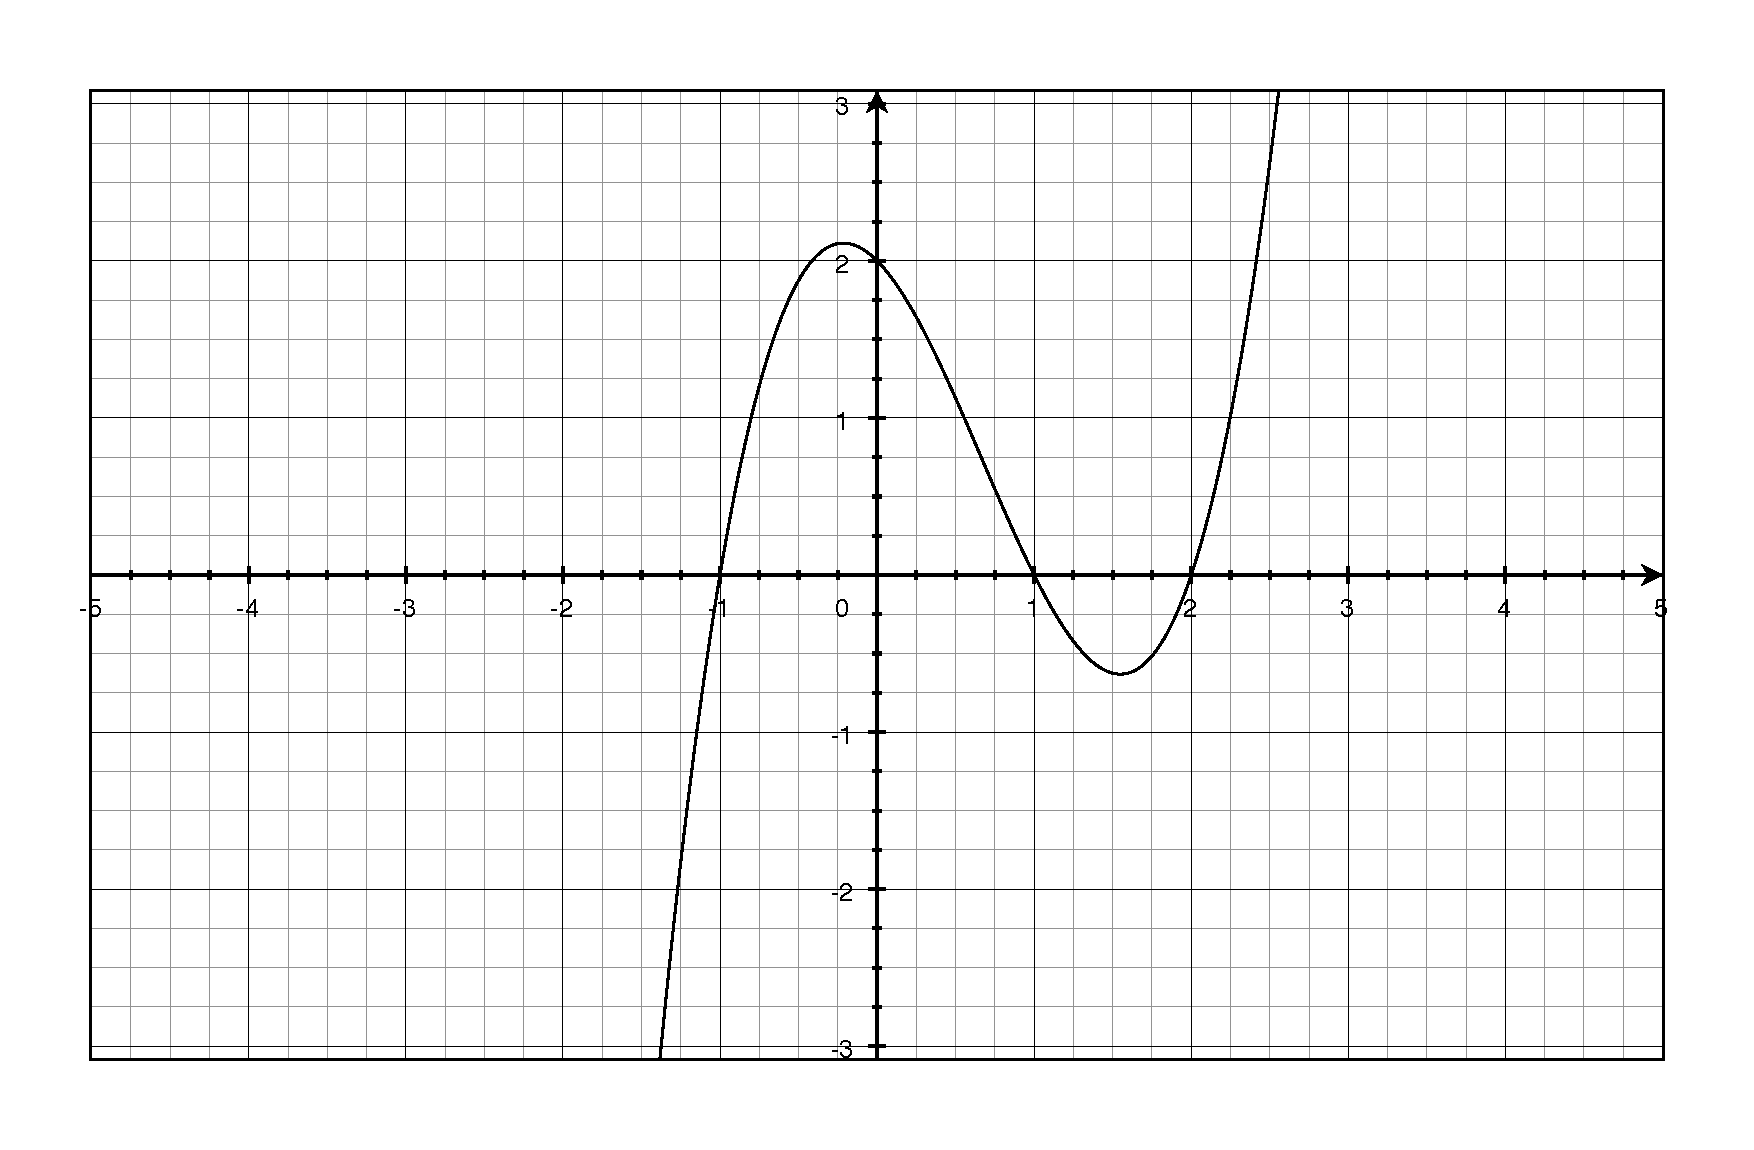
\includegraphics[width=14cm,height=10cm]{question_1.eps}
  \caption*{Question 1}
\end{figure}

\end{solution}

\ifprintanswers
\pagebreak
\else
\fi

\question $P(x) = x(x-3)(x+2)$
\begin{solution}

The zeros are: $x = \{ -2, 0, 3 \}$.

A few points:
\begin{tabular}{|c|c|c|c|c|c|}
\hline
  x & -3  & -1 &  1 & 2  & 4 \\
\hline
  y & -18 & 4 & -6 & -8 & 24 \\
\hline
\end{tabular}

\begin{figure}[H]
  \centering
  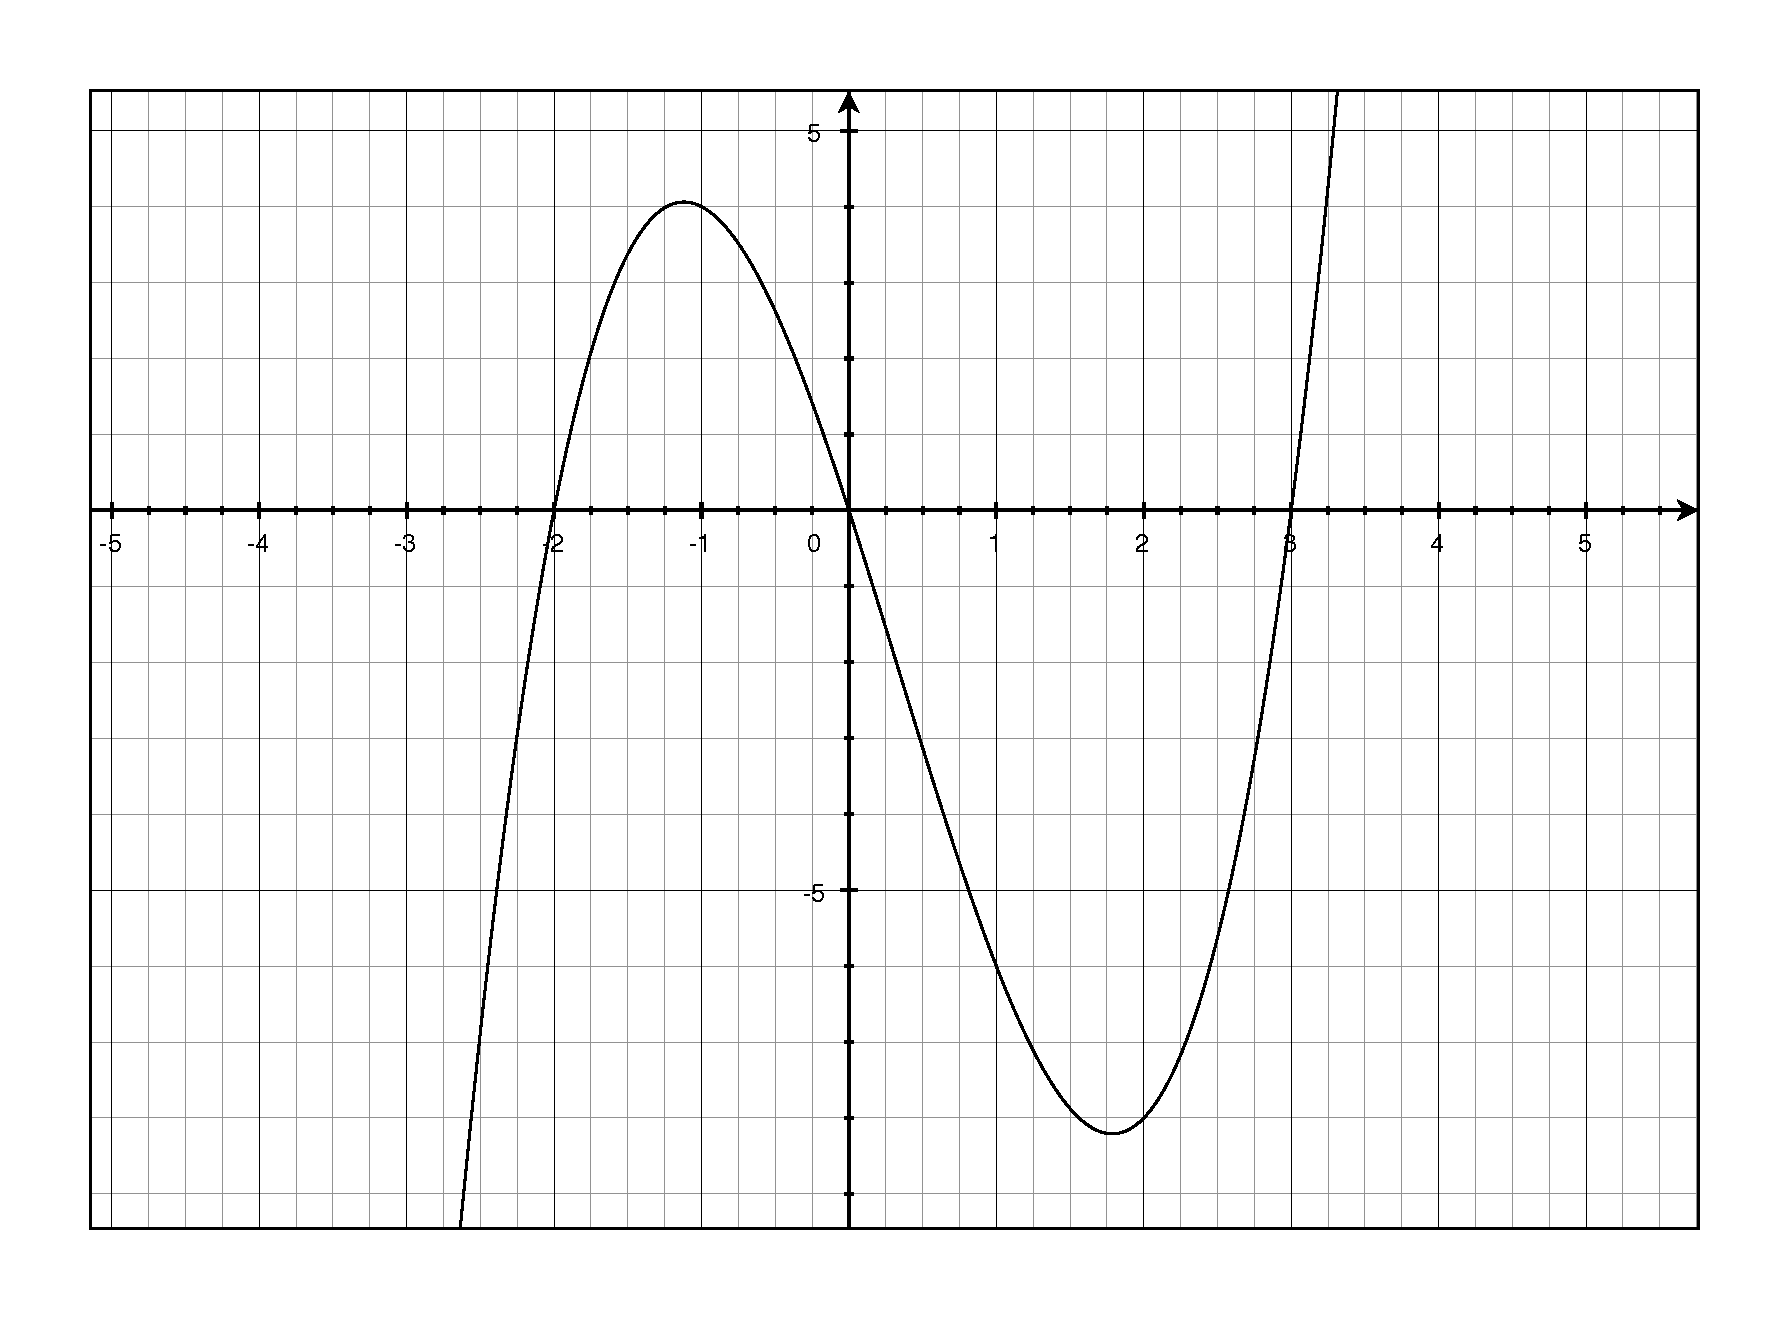
\includegraphics[width=14cm,height=10cm]{question_2.eps}
  \caption*{Question 2}
\end{figure}

\end{solution}

\question $P(x) = x(x-3)(x+2)$
\begin{solution}
see question 2
\end{solution}

\ifprintanswers
\pagebreak
\else
\fi

\question $P(x) = (x-3)(x+2)(3x-2)$
\begin{solution}

The zeros are: $x = \left\{-2, \dfrac{2}{3}, 3 \right\}$.

A few points:
\begin{tabular}{|c|c|c|c|c|c|}
\hline
  x & -1 &  0 &  1 & 2  & 4 \\
\hline
  y & 20 & 12 & -6 & -16 & 60 \\
\hline
\end{tabular}

\begin{figure}[H]
  \centering
  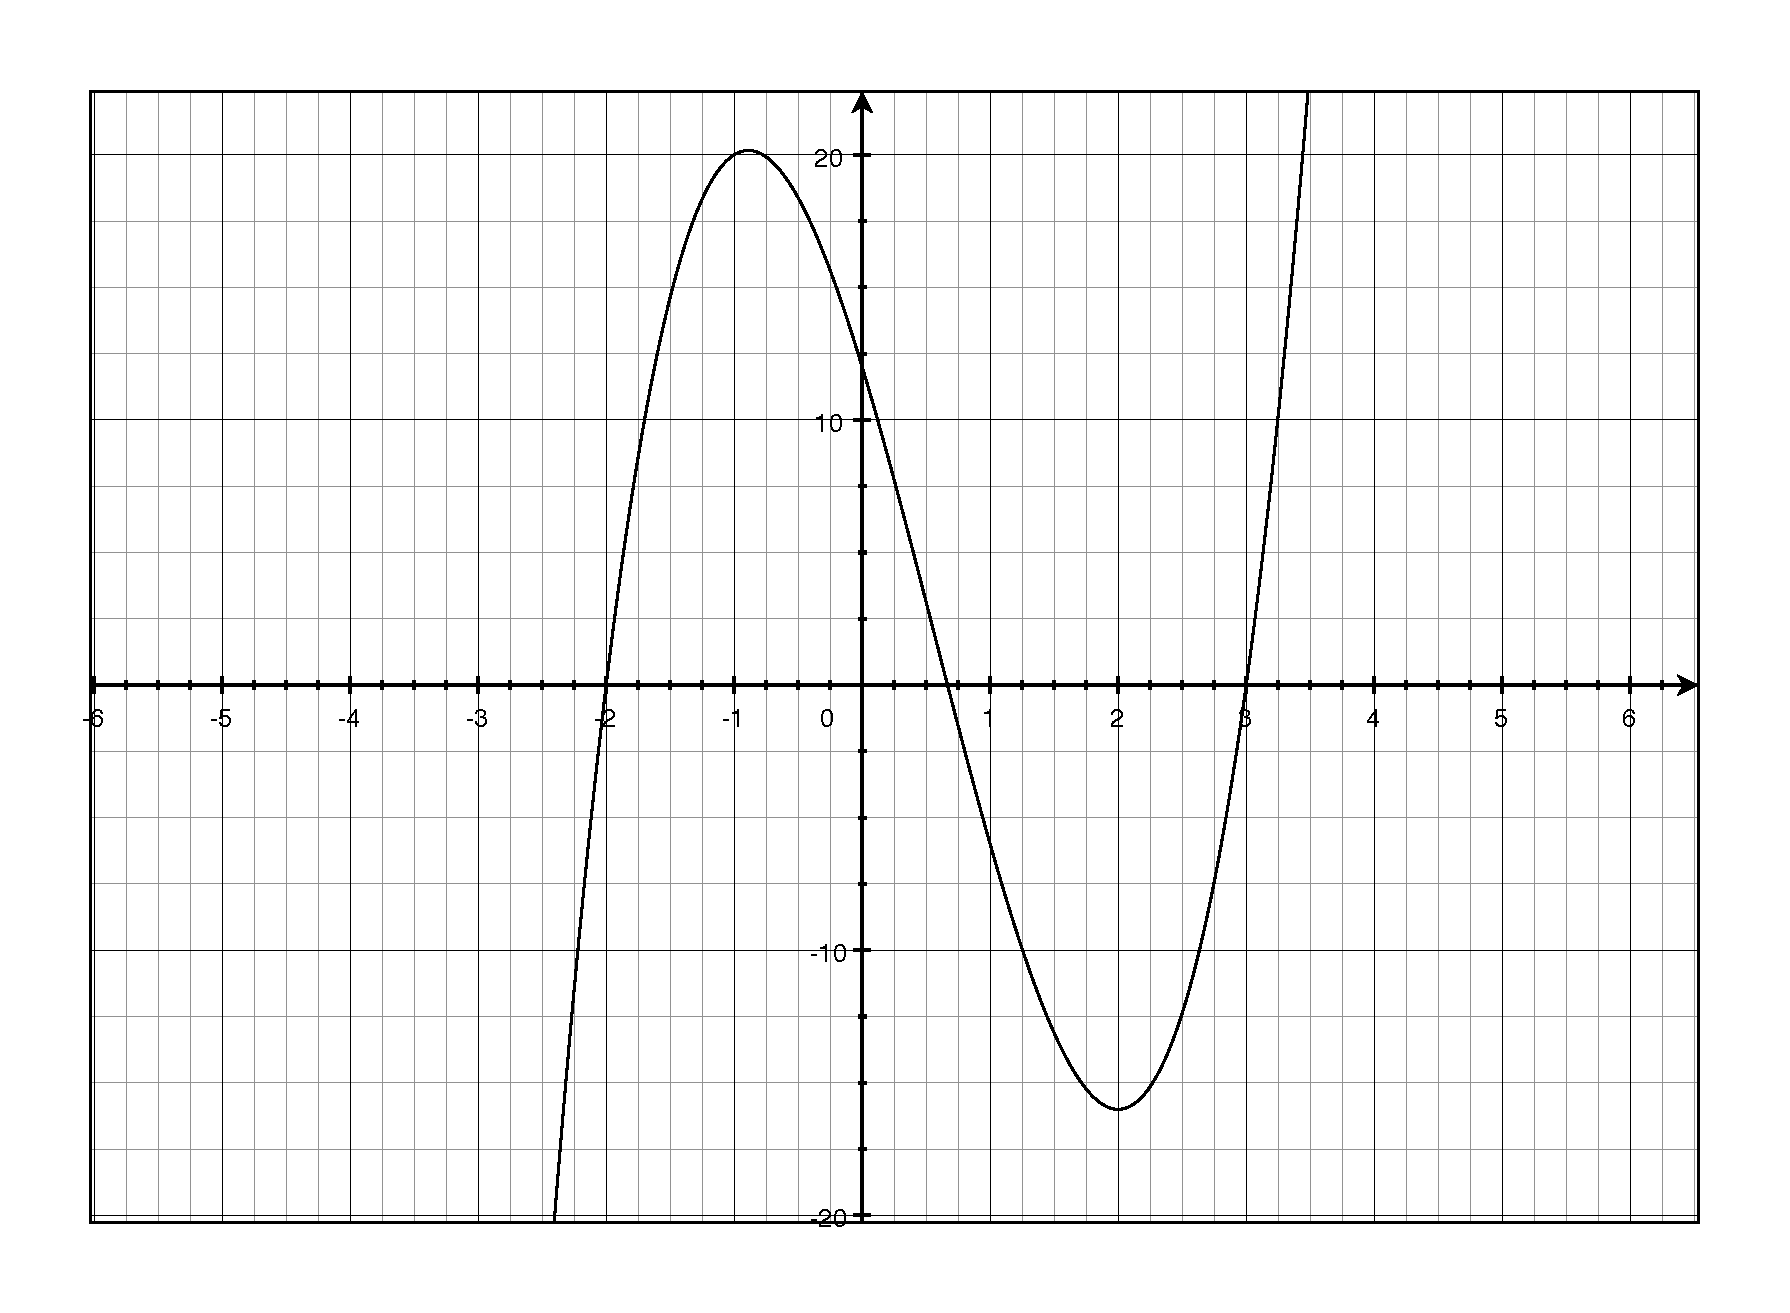
\includegraphics[width=14cm,height=10cm]{question_4.eps}
  \caption*{Question 4}
\end{figure}

\end{solution}

\ifprintanswers
\pagebreak
\else
\fi

\question $P(x) = (x-1)^2(x-3)$

\begin{solution}

The zeros are: $x = \{1, 3\}$.  The zero at $(1, 0)$ has multiplicity 2.  Since 2 is even, the graph touches but doesn't
cross the x-axis at this point.

A few points:
\begin{tabular}{|c|c|c|c|c|}
\hline
  x & -1  &  0 &  2 & 4 \\
\hline
  y & -16 & -3 & -1 & 9 \\
\hline
\end{tabular}

\begin{figure}[H]
  \centering
  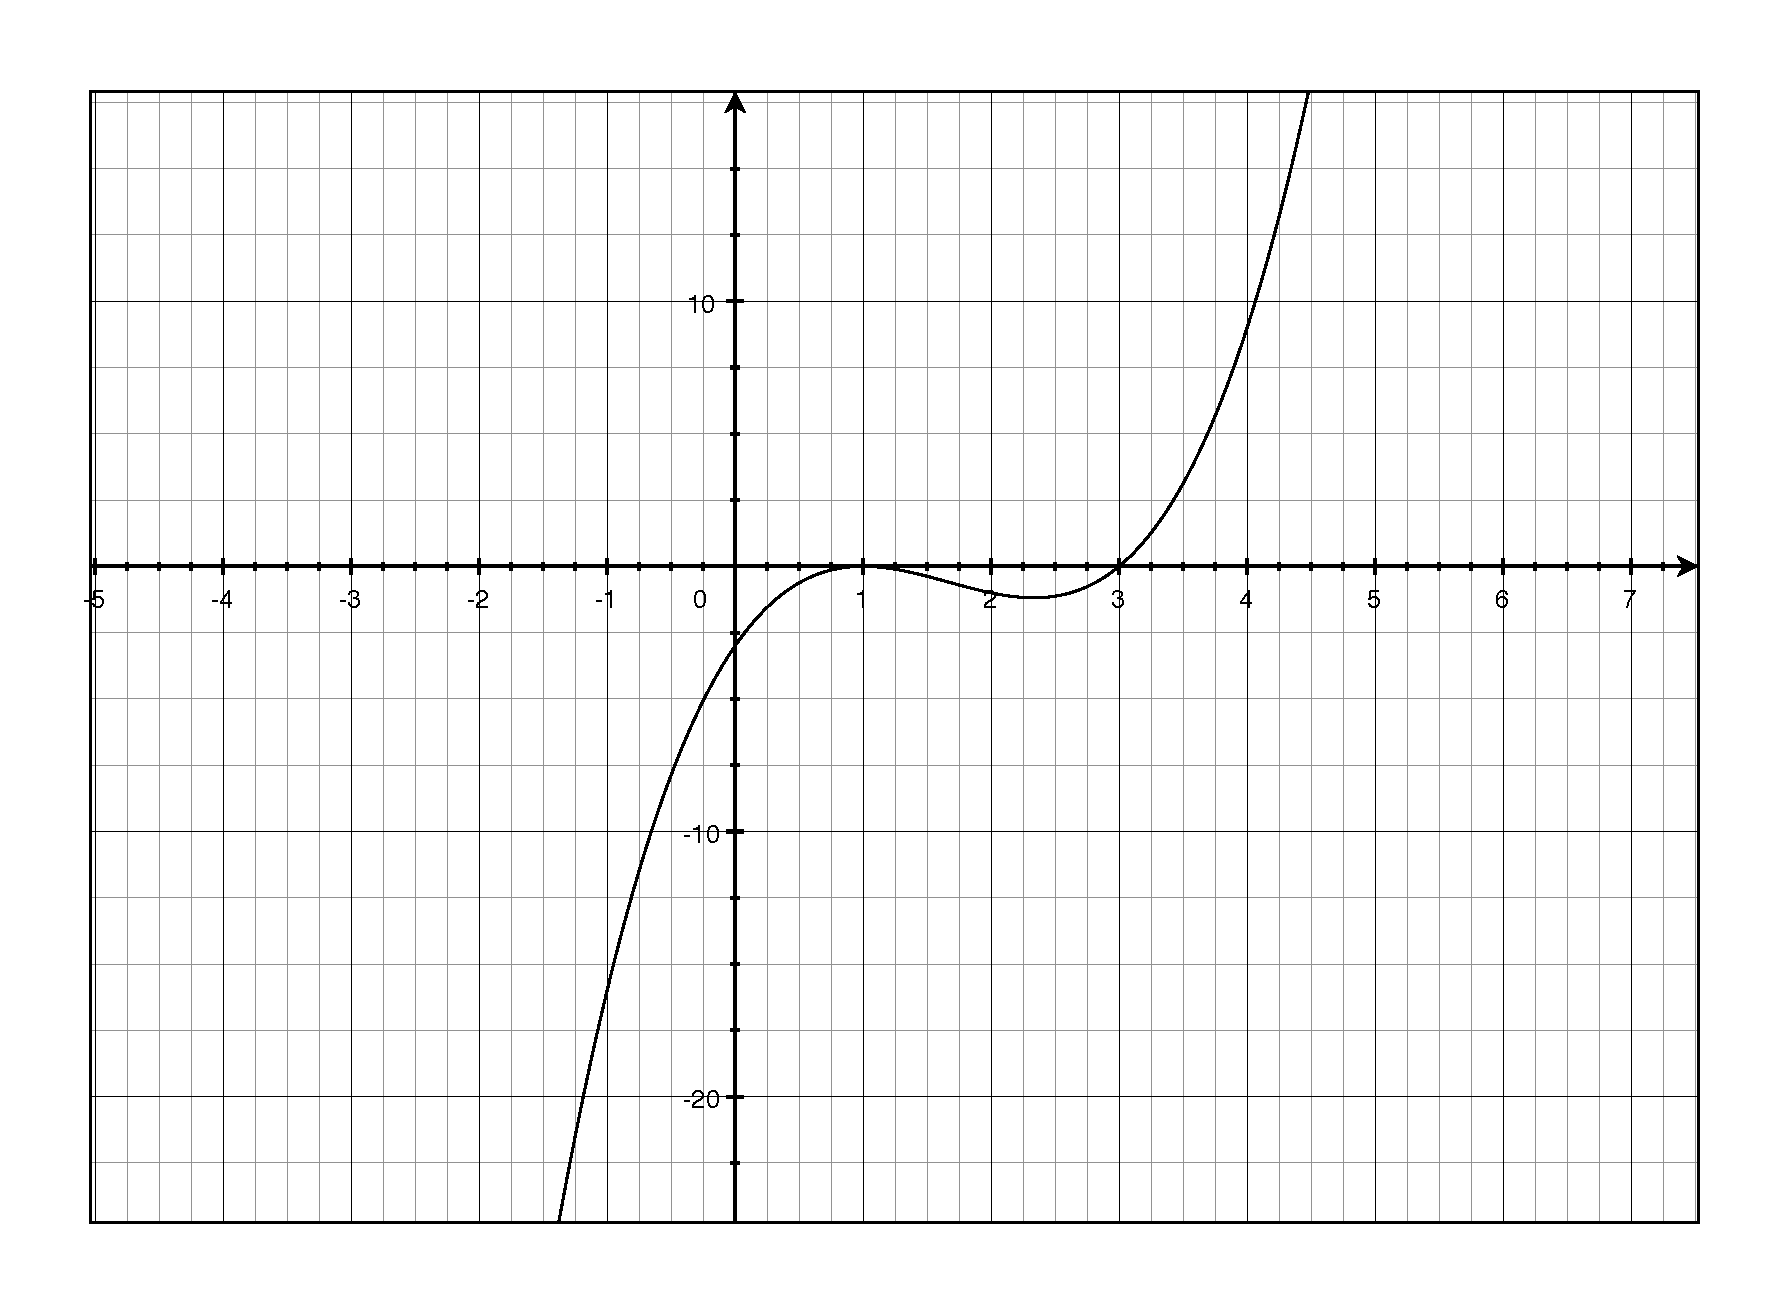
\includegraphics[width=14cm,height=10cm]{question_5.eps}
  \caption*{Question 5}
\end{figure}

\end{solution}

\ifprintanswers
\pagebreak
\else
\fi

\question $P(x) = (x-3)^2(x+1)^2$
\label{graph:last} 

\begin{solution}

The zeros are: $x = \{-1, 3\}$.  Both zeros have multiplicity 2.  Since 2 is even, the graph touches but doesn't
cross the x-axis at either of them.  

A few points:
\begin{tabular}{|c|c|c|c|c|c|}
\hline
  x & -2  & 0 &  1 & 2 & 4 \\
\hline
  y & 25  & 9 & 16 & 9 & 25 \\
\hline
\end{tabular}

\begin{figure}[H]
  \centering
  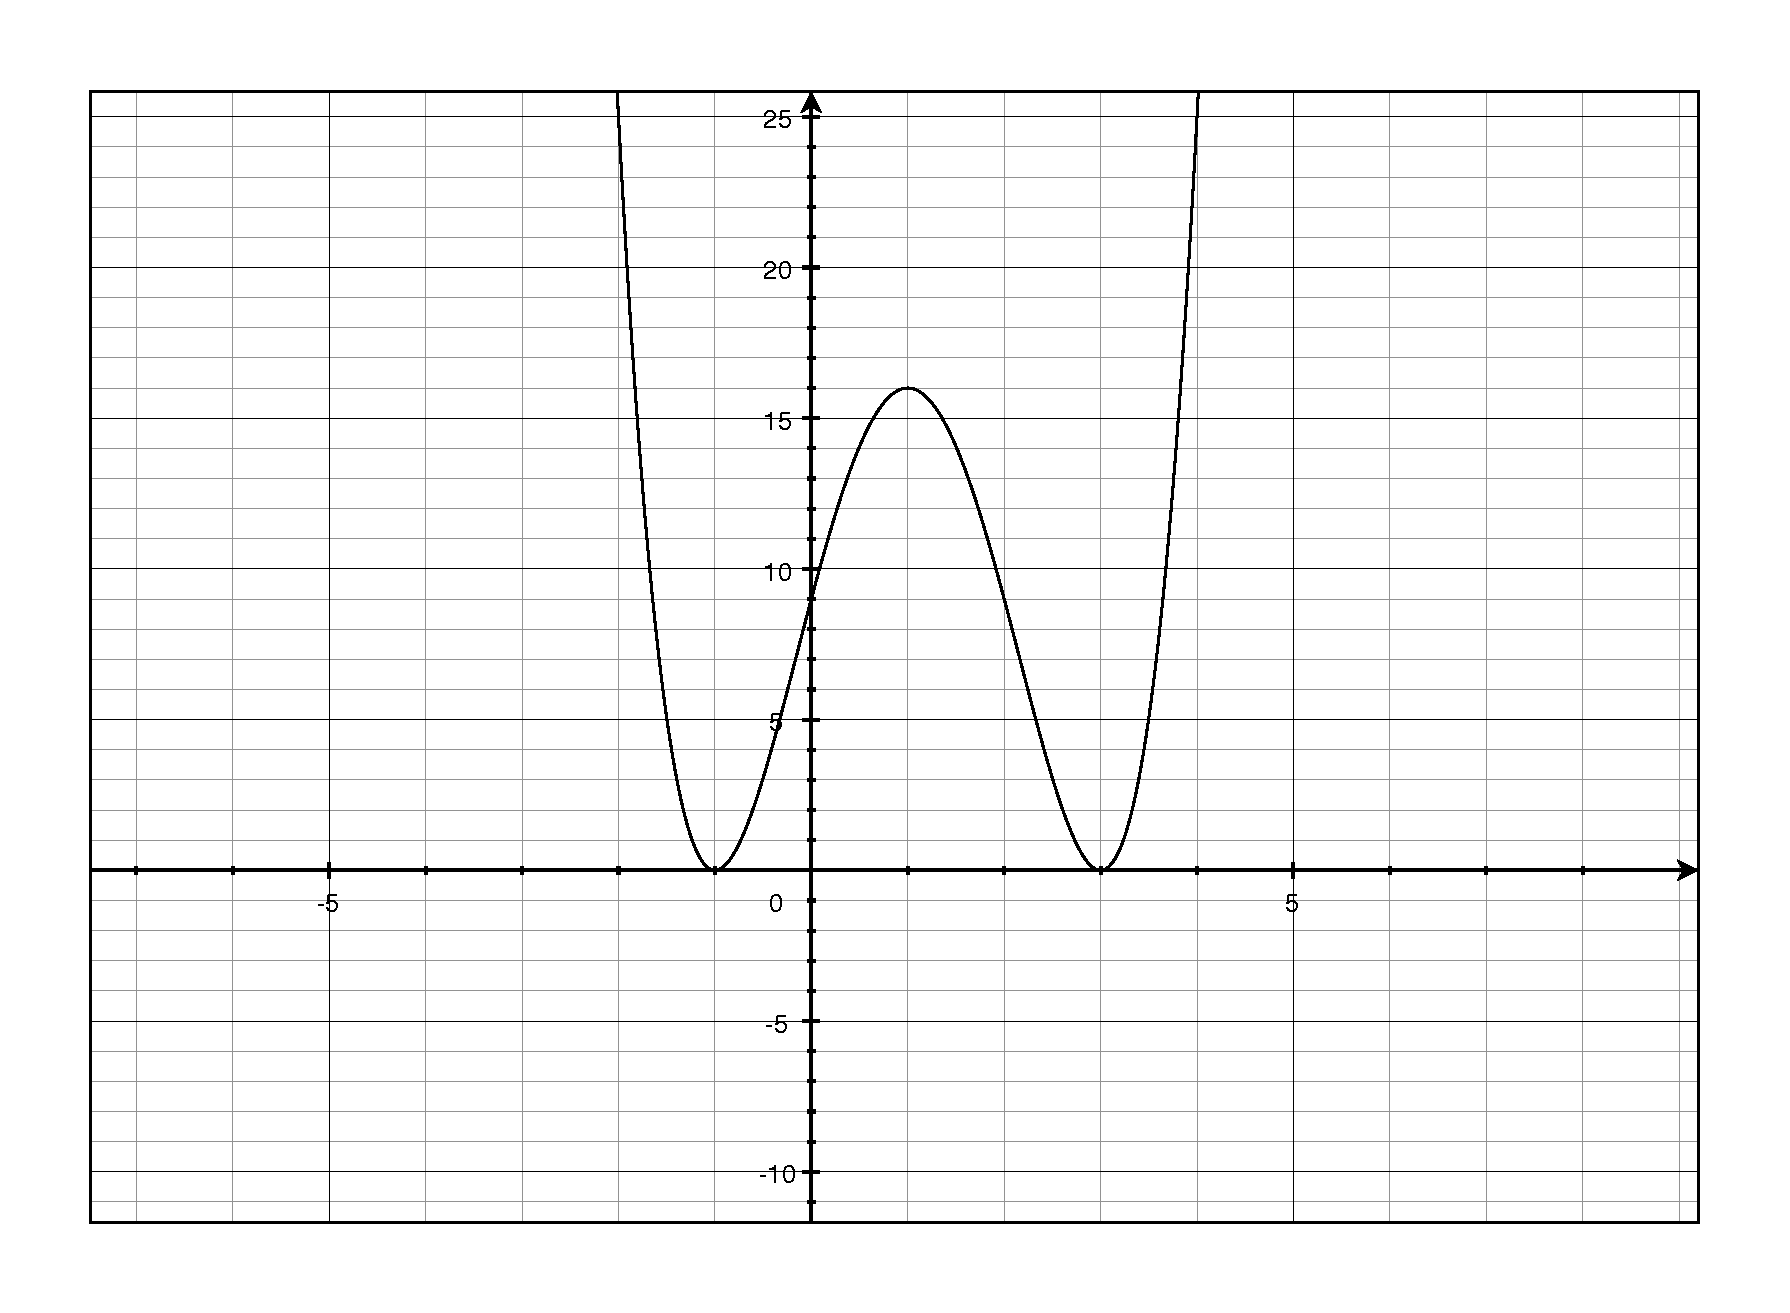
\includegraphics[width=14cm,height=10cm]{question_6.eps}
  \caption*{Question 6}
\end{figure}

\end{solution}
 
For problems \ref{factor:first}-\ref{factor:last}, factor the polynomial and use the factored form to find the zeros.
Then sketch the graph.

\question  $P(x) = x^3 - x^2 - 6x$
\label{factor:first}
\begin{solution}

\begin{align*}
  P(x) &= x^3 - x^2 - 6x \\
       &= x(x^2 - x - 6) \\
       &= x(x-3)(x+2) \\
\end{align*}

I must have really liked this equation, as after factoring, this one is the same as problems 2 and 3.

\end{solution}

\ifprintanswers
\pagebreak
\else
\fi

\question $P(x) = -x^3+x^2+12x$
\begin{solution}

\begin{align*}
  P(x) &= -x^3+x^2+12x \\
   &= -x(x^2-x-12) \\
   &= -x(x-4)(x+3) \\
\end{align*}

The zeros are: $x = \{-3, 0, 4\}$

A few points:
\begin{tabular}{|c|c|c|c|c|c|c|c|}
\hline
  x & -4 & -1  & -2  & 0 & 1  & 3 & 5 \\
\hline
  y & 32 & -10 & -16 & 0 & 12 & 18 & -20 \\
\hline
\end{tabular}

\begin{figure}[H]
  \centering
  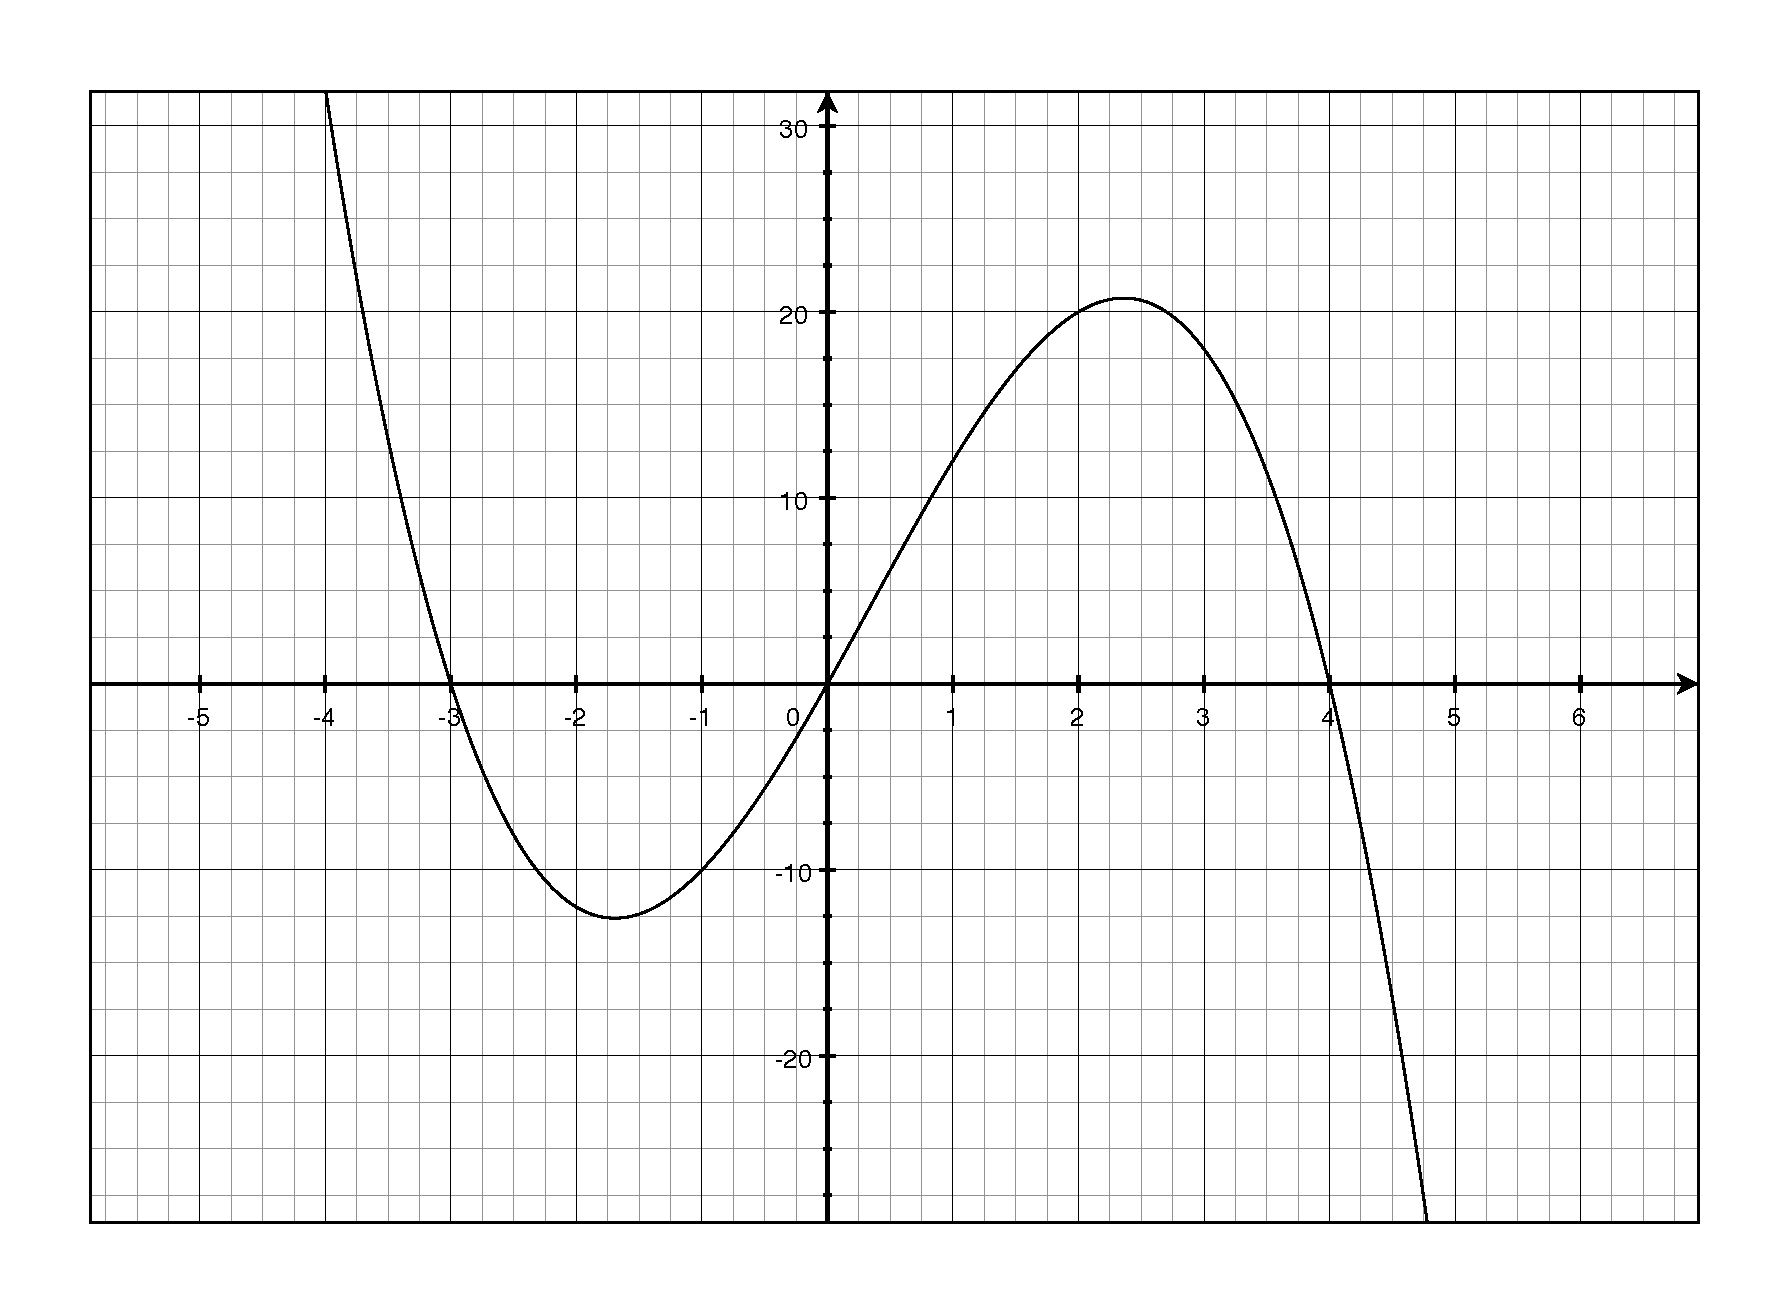
\includegraphics[width=14cm,height=10cm]{question_8.eps}
  \caption*{Question 8}
\end{figure}

\end{solution}

\ifprintanswers
\pagebreak
\else
\fi

\question $P(x) = -2x^3-x^2+x$
\begin{solution}

The zeros are: $x = \left\{ -1, 0, \dfrac{1}{2} \right\}$.  

A few points:
\begin{tabular}{|c|c|c|c|c|}
\hline
  x & $-2$ & $-1/2$ & $1/4$  &  2  \\
\hline
  y & 10   & $-1/2$ & $5/32$ & -18 \\
\hline
\end{tabular}

\begin{figure}[H]
  \centering
  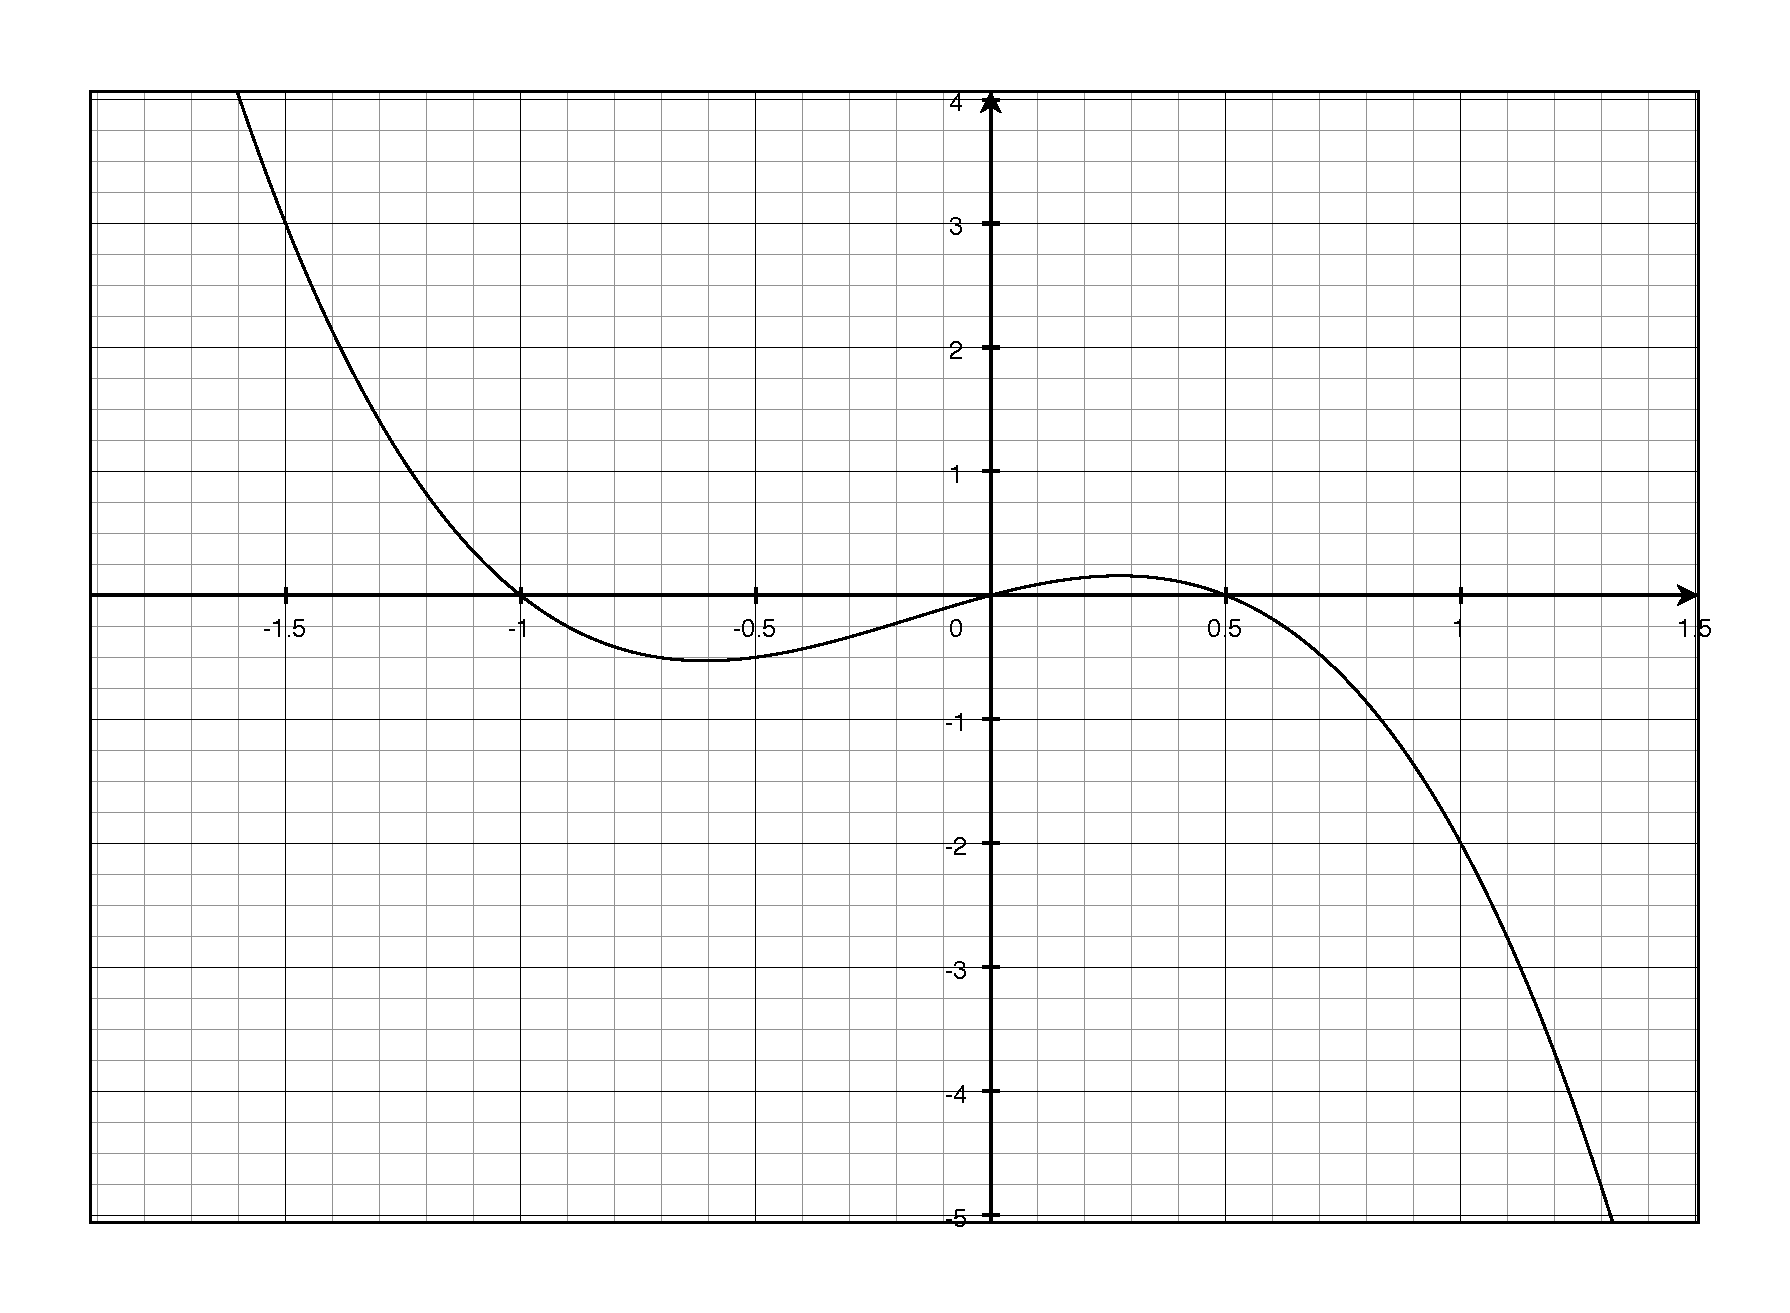
\includegraphics[width=14cm,height=10cm]{question_9.eps}
  \caption*{Question 9}
\end{figure}

\end{solution}

\ifprintanswers
\pagebreak
\else
\fi

\question $P(x) = x^4-3x^3+2x^2$
\label{factor:last} 
\begin{solution}
\begin{align*}
  P(x) &= x^4-3x^3+2x^2 \\
  &= x^2(x^2-3x+2) \\
  &= x^2(x-2)(x-1) \\
\end{align*}

The zeros are: $x = \{0, 1, 2 \}$.

A few points:
\begin{tabular}{|c|c|c|c|}
\hline
  x & -1 & $1/2$ & $3/2$   \\
\hline
  y & 6 & $3/16$ & $-9/16$ \\
\hline
\end{tabular}

\begin{figure}[H]
  \centering
  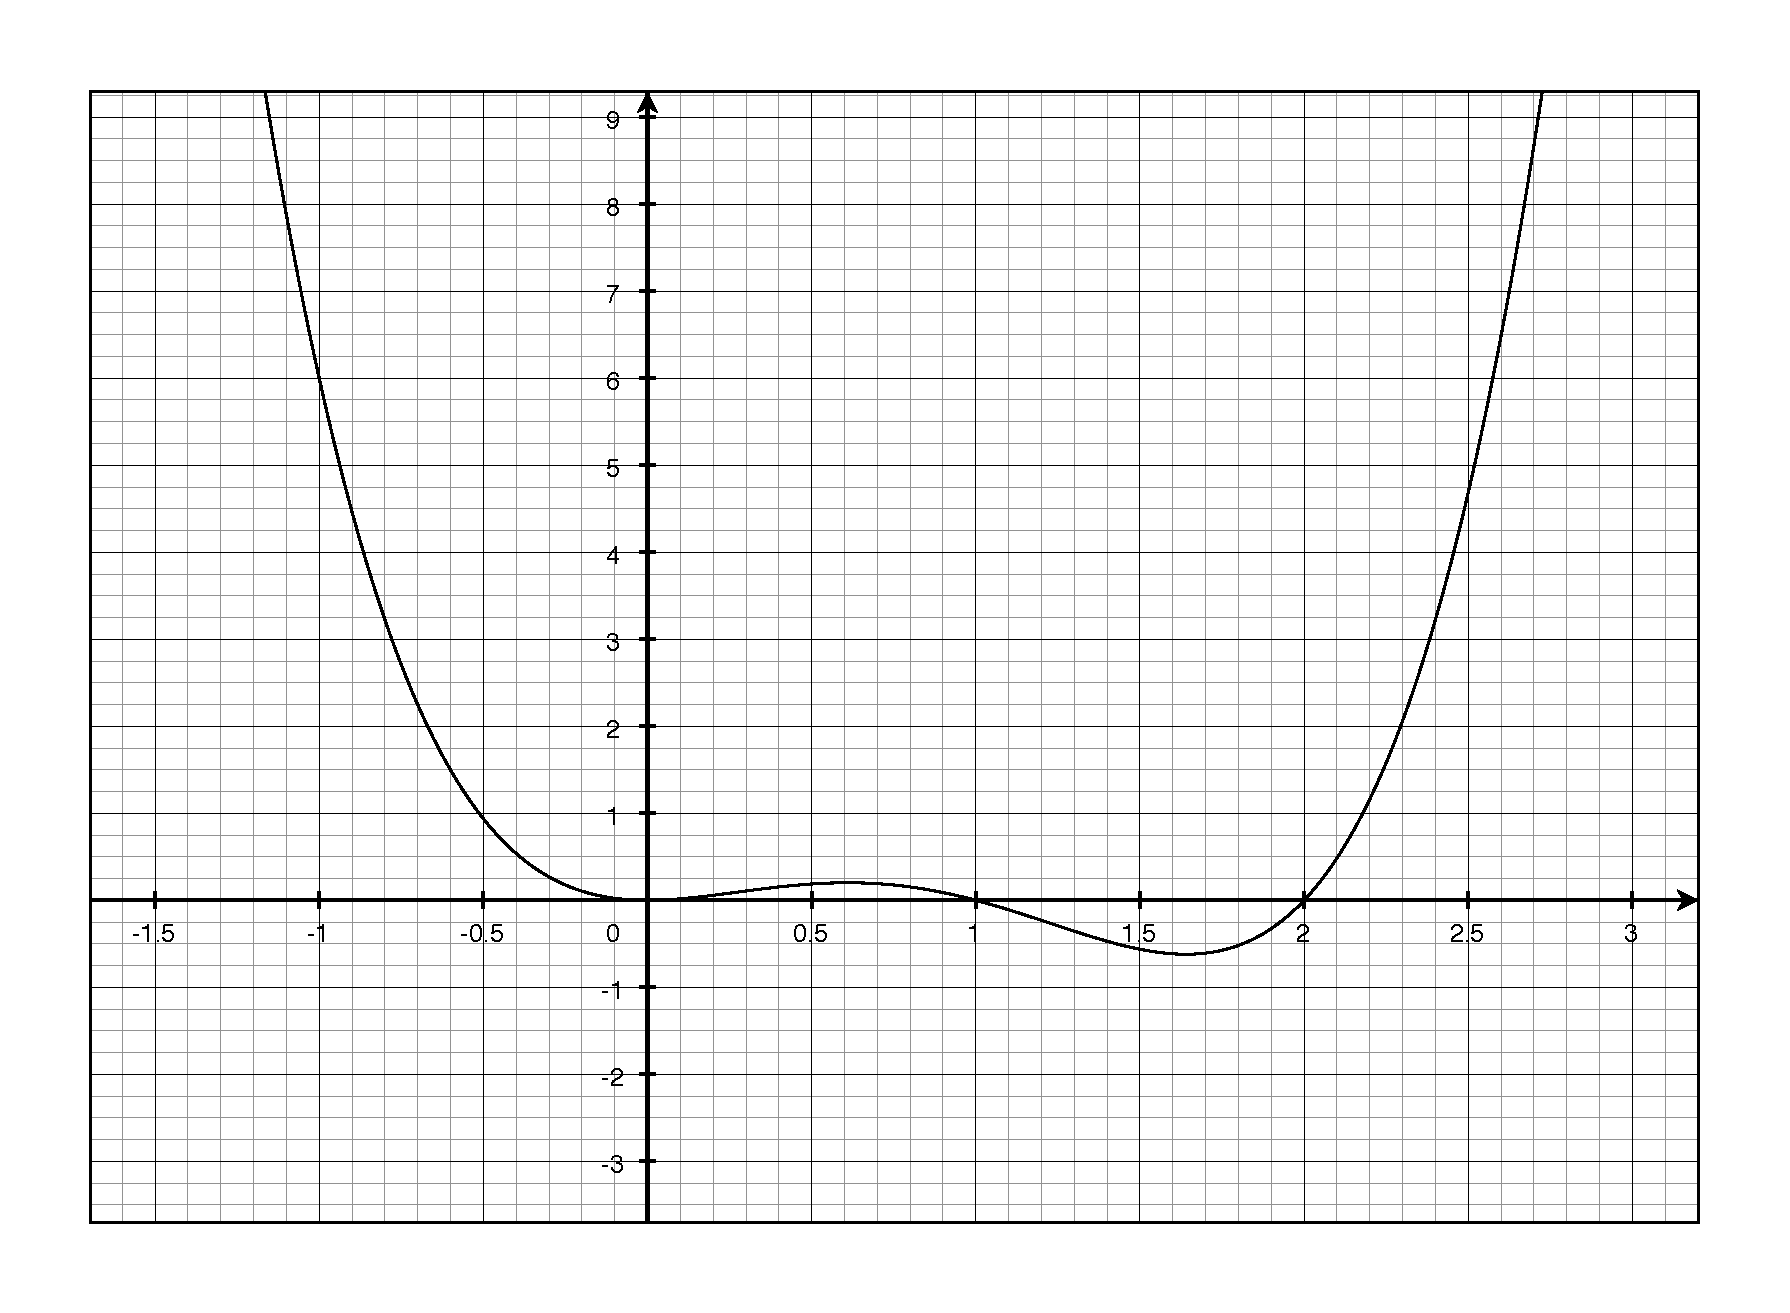
\includegraphics[width=14cm,height=10cm]{question_10.eps}
  \caption*{Question 10}
\end{figure}

\end{solution}

\section{Calculator Problems}

Do problems \ref{calculator:first} - \ref{calculator:last}, if you can get to the PAB to borrow a calculator.  

For problems \ref{calculator:first}-\ref{compare:last}, determine the end behavior of $P$.  Compare the graphs of $P$ and
$Q$ on large and small viewing rectangles.  There is nothing to hand in for these.

\question
\label{calculator:first}
\begin{align*}  
  P(x) &= -\frac{1}{8}x^3 + \frac{1}{4}x^2 + 12x \\
  Q(x) &= -\frac{1}{8}x^3 \\
\end{align*}

\question
\begin{align*}
  P(x) &= x^{11} - 9x^9\\
  Q(x) &= x^{11} \\
\end{align*}

\question
\label{compare:last}
\begin{align*}
  P(x) &= -x^{12} + 2x^2\\
  Q(x) &= -x^{12} \\
\end{align*}

For problems \ref{extrema:first}-\ref{calculator:last}, graph the polynomial and find the coordinates of all local
extrema.

\question \label{extrema:first} $f(x) = x^3 - 12x + 9$
\begin{solution}
extrema: $(-2, 25)$ and $(2, -7)$
\begin{figure}[H]
  \centering
  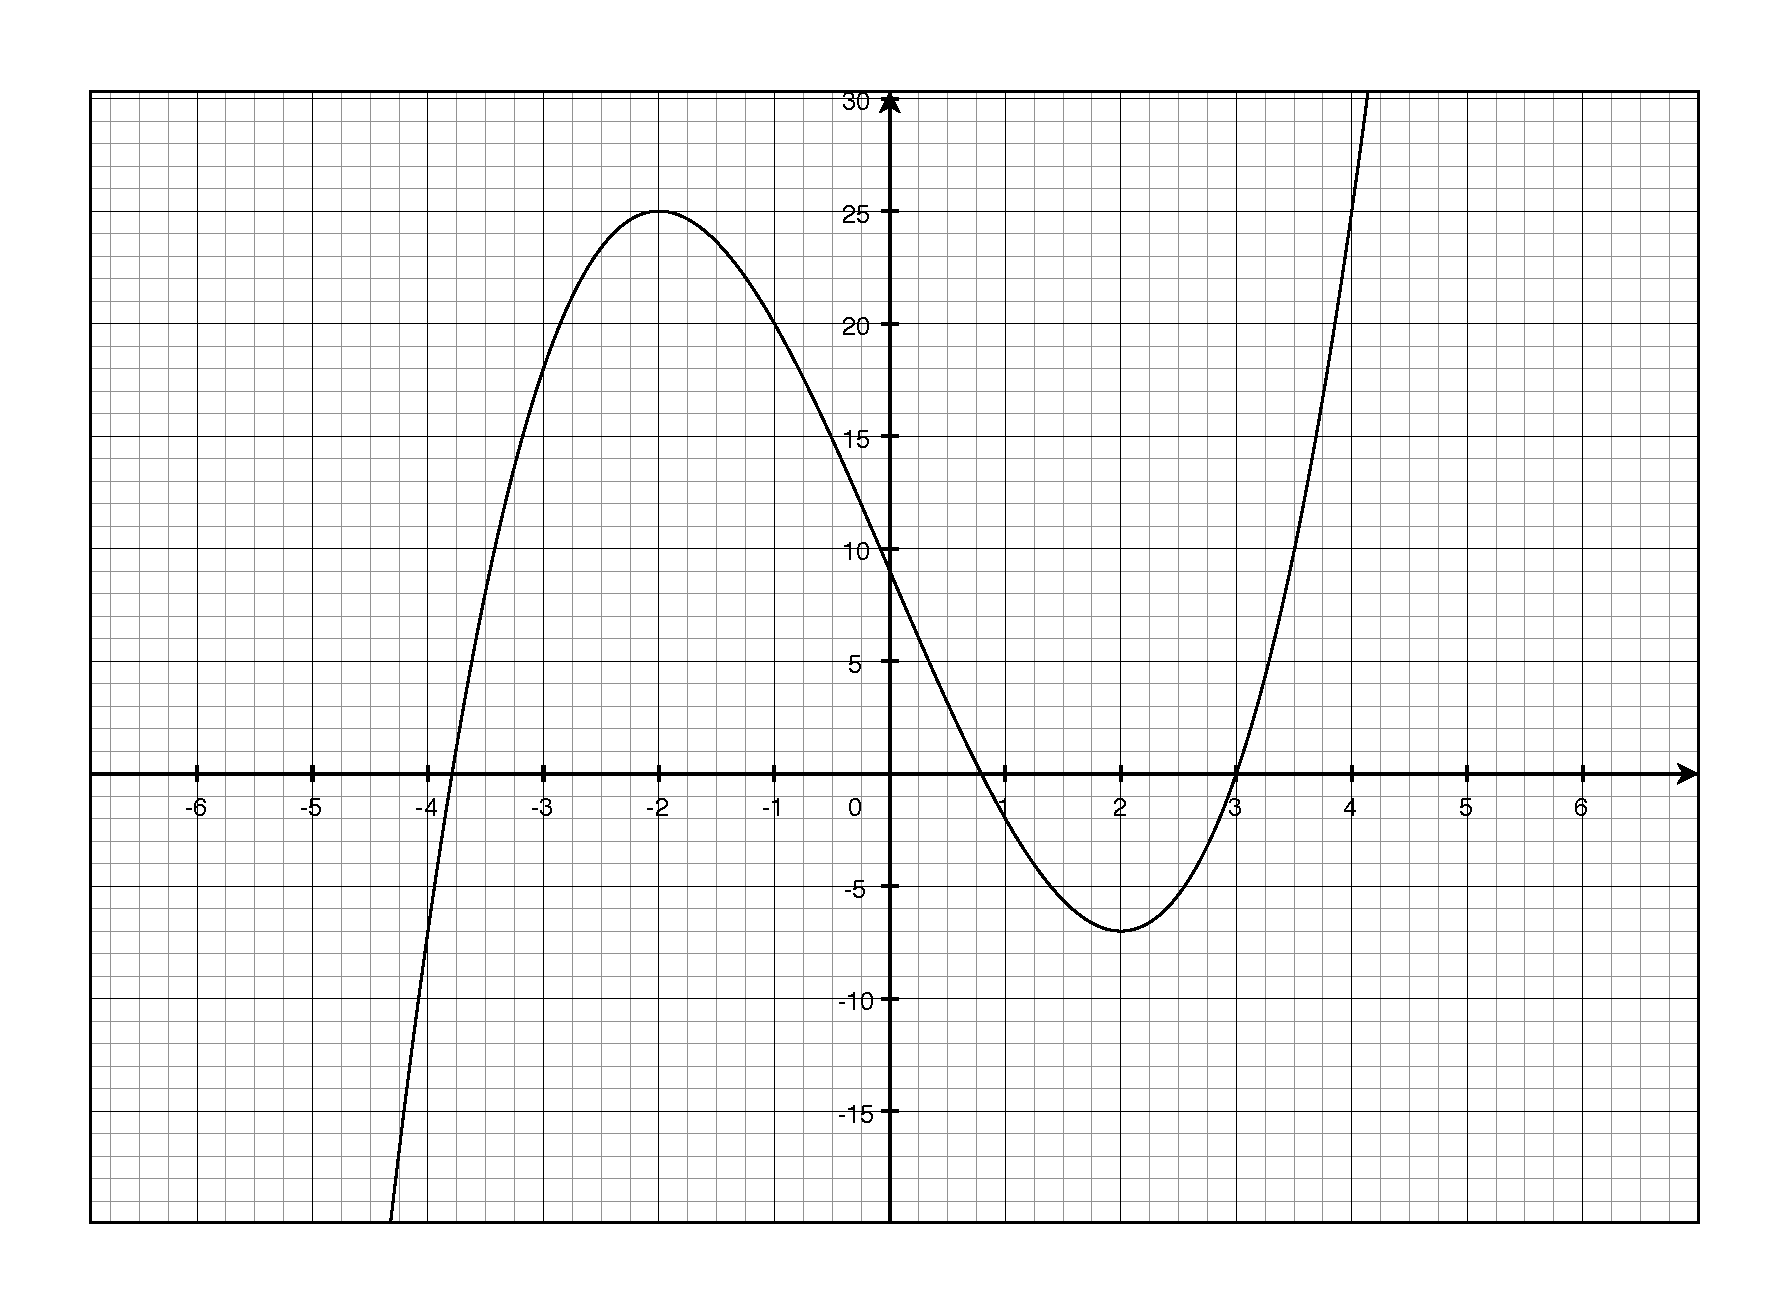
\includegraphics[width=14cm,height=10cm]{question_11.eps}
  \caption*{Question 11}
\end{figure}

\end{solution}

\ifprintanswers
\pagebreak
\else
\fi

\question  $f(x) = 3x^5-5x^3+3$

\begin{solution}
extrema: $(-1, 5)$, $(1, 1)$
\begin{figure}[H]
  \centering
  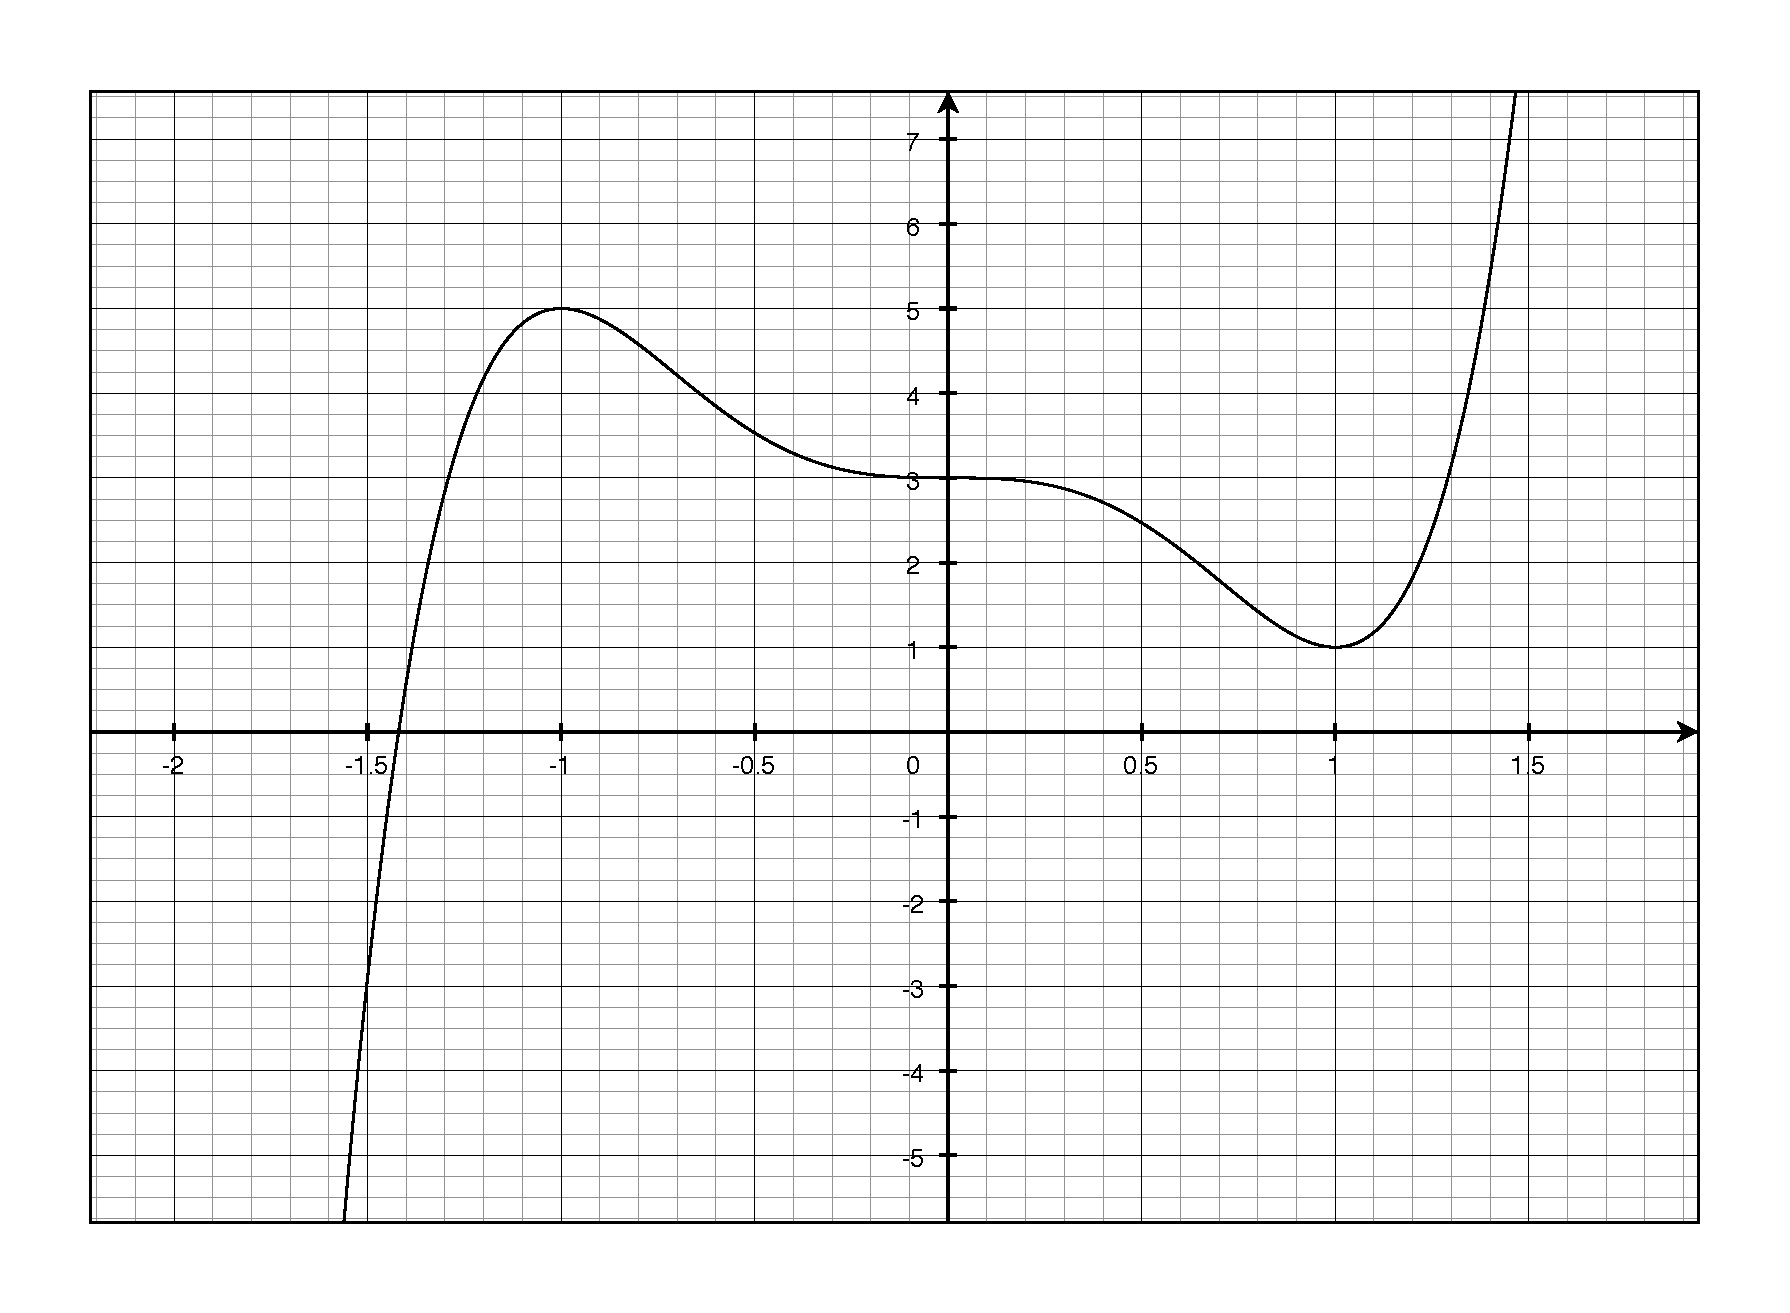
\includegraphics[width=14cm,height=10cm]{question_15.eps}
  \caption*{Question 15}
\end{figure}

\end{solution}

\ifprintanswers
\else
\pagebreak
\fi

\question \label{calculator:last} $f(x) = x^5-5x^2+6$
\begin{solution}
extrema: $(0, 6)$, $(1.2598, 1.2378)$
\begin{figure}[H]
  \centering
  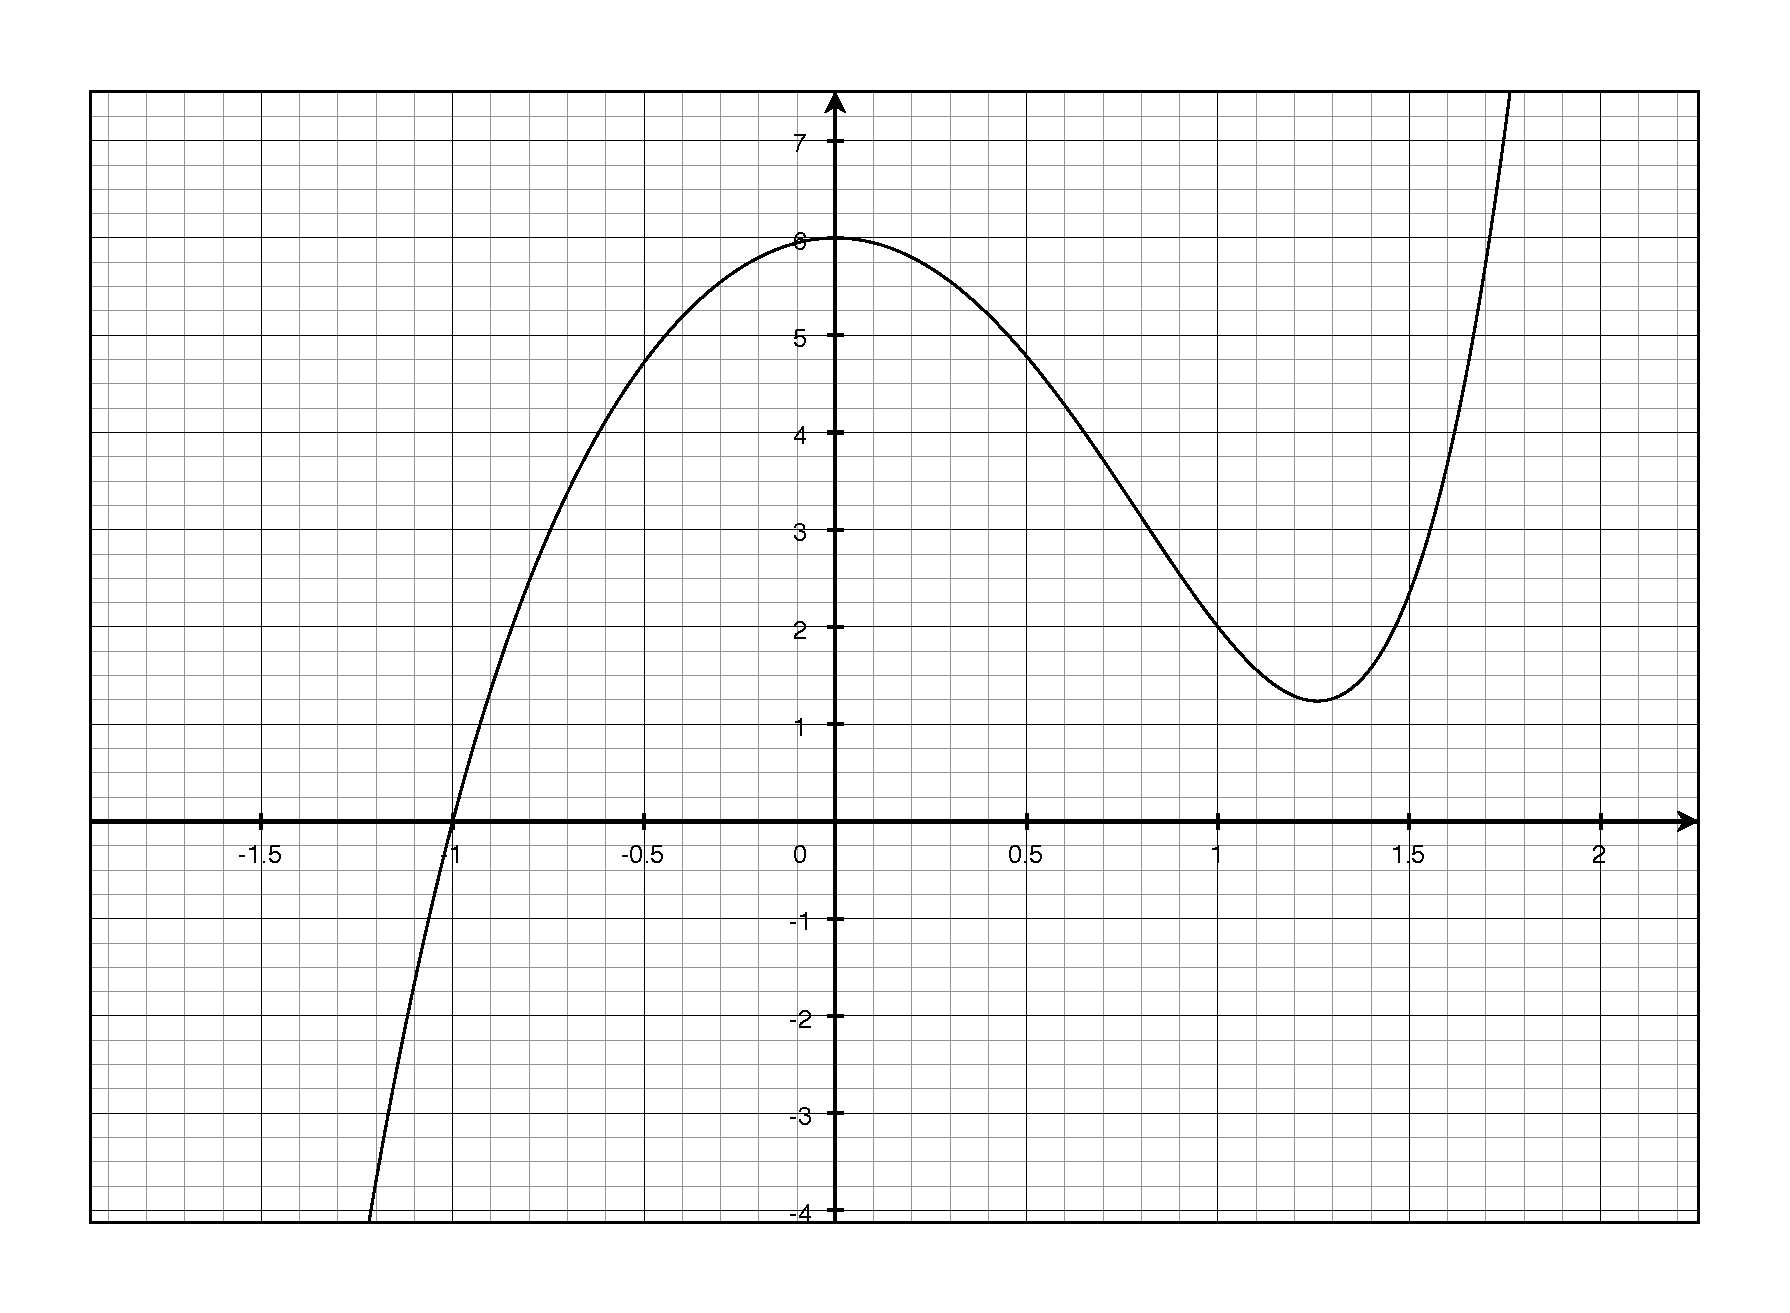
\includegraphics[width=14cm,height=10cm]{question_16.eps}
  \caption*{Question 16}
\end{figure}

\end{solution}

\end{questions}

\section{Extra Credit}

These questions refer to the story below.
\begin{questions}

\question 
If Emile sends $n$ gifts on day $n$, find a function $g(n)$ which gives the total number of gifts received so far
(counting all the previous days) on day $n$. 

\begin{solution}
To find the equation, you have to notice that you can split the numbers into pairs starting from the first and last day and
working towards the middle.  For example, on day 8, you have :
\begin{itemize}
  \item 1 and 8
  \item 2 and 7
  \item 3 and 6
  \item 4 and 5
\end{itemize}


For this day, there are 4 pairs and each pair adds up to 9.  The same approach would work for any even numbered day.
So for even numbered days, you have $\dfrac{n}{2}$ pairs and each pair adds up to $n+1$.  So for even numbered days, the
correct function is:
\[
  g(n) = \left( \frac{n}{2} \right) \cdot (n+1) = \frac{n(n+1)}{2}
\]

For odd numbered days, you have one number, or half of a pair, left over in the middle.  This works out fine, because
$\dfrac{n}{2}$ is a fraction for odd numbers, so the same function also works for odd numbered days.

Here are all the values from the domain:

\begin{tabular}{|c|c|c|c|c|c|c|c|c|c|c|c|c|}
\hline
  $n$ (day)                & 1 & 2 & 3 & 4 & 5  & 6   & 7 & 8  & 9 & 10 & 11 & 12 \\
\hline
  $g(n)$ (number of gifts) & 1 & 3 & 6 & 10 & 15 & 21 & 28 & 36 & 45 & 55 & 66 & 78 \\
\hline
\end{tabular}

\end{solution}
\question

Find $g^{-1}(n)$.  What does it represent?

\begin{solution}

\begin{align*}
  y &= \frac{n(n+1)}{2} \\
  y  &= \frac{n^2+n}{2} \\
  2y  &= n^2+n \\
  n^2+n -2y &= 0 \\
\end{align*}

This equation doesn't factor, so we need to use the quadratic equation to solve for $n$.

\[
  n = \frac{-1 \pm \sqrt{1 - 4(-2y)}}{2} = \frac{-1 \pm \sqrt{1 + 8y}}{2}
\]

Negative values don't make sense for this function, so the final inverse function is:
\[
  g^{-1}(n) = \frac{-1 + \sqrt{1 + 8n}}{2}
\]

Since original function provided the total number of gifts sent by Emile by day $n$, this function provides the day on
which Emile will have sent $n$ total gifts.  The domain for this function is the range of the original function.

Here are all the values from the domain:

\begin{tabular}{|c|c|c|c|c|c|c|c|c|c|c|c|c|}
\hline
  $n$ (number of gifts)    & 1 & 3 & 6 & 10 & 15 & 21 & 28 & 36 & 45 & 55 & 66 & 78 \\
\hline
  $g^{-1}(n)$  (day number) & 1 & 2 & 3 & 4 & 5  & 6   & 7 & 8  & 9 & 10 & 11 & 12 \\
\hline
\end{tabular}

Since this is the inverse of $g(n)$, the table is the same with different labels for the rows.
\end{solution}
 
\end{questions}

\ifprintanswers
\else

\makebox[\textwidth]\hrulefill

\begin{description}
\item[Day 1].

Dear Emile,

Thanks for da bird in the Pear tree. I fixed it las night with dirty rice an' it was delicious. I doan tink the Pear
tree would grow in de swamp, so I swapped it for a Satsuma.

\item[Day 2].

Dear Emile,

Your letter said you sent 2 turtle dove, but all I got was 2 scrawny pigeon. Anyway, I mixed them with andouille and
made some gumbo out of dem.

\item[Day 3].

Dear Emile,

Why doan you sen me some crawfish? I'm tired of eating dem darned bird. I gave two of those prissy French chicken to
Mrs. Fontenot over at Grand Chenier, and fed the tird one to my dog, Phideaux. Mrs. Fontenot needed some sparring
partners for her fighting rooster.

\item[Day 4].

Dear Emile,

Mon Dieux! I tole you no more of dem bird. Deez four, what you call ``calling bird'' wuz so noisy you could hear dem all
da' way to Lafayette. I used they necks for my crab traps, and fed the rest of dem to the gators.

\item[Day 5].

Dear Emile,

You finally sent something useful. I liked dem golden rings, me. I hocked dem at da' pawn shop in Sulphur and got enough
money to fix the shaft on my shrimp boat, and to buy a round for da boys at the Raisin' Cane Lounge. Merci Beaucoup!

\item[Day 6].

Dear Emile,

Couchon! Back to da birds, you big dumb turkey! Poor egg sucking Phideaux is scared to death ah dem six goose. He try to
eat they eggs and they pecked the heck out ah his snout. Dem goose are dang good at eating cockroach around da' house,
though. I may stuff one ah dem goose with erster dressing to serve him on Christmas Day.

\item[Day 7].

Dear Emile,

I'm gonna wring your fool neck next time I see you. Ole Boudreaux, da mailman, is ready to kill you, too. The poop from
all dem bird is stinkin up his mailboat. He afraid someone will slip on dat stuff and gonna sue him. I let dem seven
swan loose to swim on da bayou and some stupid duck hunter from Mississippi done blasted dem out da water. Talk to you
tomorrow.

\item[Day 8].

Dear Emile,

Poor ole Boudreaux had to make 3 trips on his mailboat to deliver dem 8 maids-a-milking and der cows. One of dem cows
got spooked by da alligators and almost tipped over da boat. I doan like dem shiftless maids, me. I told dem to get to
work gutting fish and sweeping my shack--but dey say it wasn't in their contract. They probably tink they too good to
skin all dem nutria I caught las night.

\item[Day 9].

Dear Emile,

What you trying to do? Boudreaux had to borrow da Cameron Ferry to carry these jumping twits you call lords-a-leaping
across da bayou. As soon as dey got here dey wanted a tea break and crumpets. I doan know what dat means but I says,
"Well la di da. You get Chicory coffee or nuthin." Mon Dieux, Emile, what I'm gonna feed all these bozos? They too
snooty for fried nutria, and da cow ate up all my turnip green.

\item[Day 10].

Dear Emile,

You got to be out of you mind. If da mailman don't kill you, I will. Today he deliver 10 half nekkid floozies from
Bourbon Street. Dey said they be "ladies dancing" but they doan act like ladies in front of dem Limey sailing boys. Dey
almost left after one of them got bit by a water moccasin over by my out- house. I had to butcher 2 cows to feed toute
le monde (everybody) and get toilet paper rolls. The Sears catalog wasn't good enough for dem hoity toity lords. Talk at
you tomorrow.

\item[Day 11].

Dear Emile,

Where Y'at? Cherio and pip pip. You 11 Pipers Piping arrived today from the House of Blues, second lining as dey got off
da boat. We fixed stuffed goose and beef jumbalaya, finished da whiskey, and we're having a fais-do-do. Da' new mailman
drank a bottle of Jack Daniel, and he's having a good old time dancing with the floozies. Da' old mailman done jump off
the Moss Bluff Bridge yesterday, screaming you name. If you happen to get a mysterious-looking, ticking package in da
mail, don't open it.

\item[Day 12].

Dear Emile,

Me I'm sorry to tell you--but I am not your true love anymore. After the fais-do-do, I talked all da night with Jacque,
the head piper. We decide to open a restaurant and gentlemen's club on the bayou. The floozies--pardon me--ladies
dancing can make \$20 un hour for dancin', and the lords can be the waiters and valet park da boats. Since da' maids
have no more cows to milk, I trained dem to set my crab traps, watch my trotlines, and run my shrimping business. We'll
probably gross a million dollars next year.

\end{description}

Joyeaux Noel et Bonne Annee!

\vspace{2 cm}

\fi

% {\em Happy Holidays!}

% \vspace{.1 cm}
% \hspace{1 cm} --Ed Tellman

\end{document}

